% !TeX spellcheck = en_US
\section{Problem 3}

Henon map is a dynamic system described by the recursive equation 
\[
x_{k+1} = 1 - ax^2_k + bx_{k-1}
\]

A lot of dynamic systems transition into chaos as gain or control is increased to a certain point and this system falls into this category.
In this problem, we will plot the trajectories of sequences $x_0 ... x_i$ and describe it.

The first parameters are (a,b) = (0.3, 0.4) and the trajectories of the sequences are presented in figure~\ref{fig:prob3_x_init}.

\begin{figure}[htpb]
	\centering
	\begin{subfigure}{.47\textwidth}
		\centering
		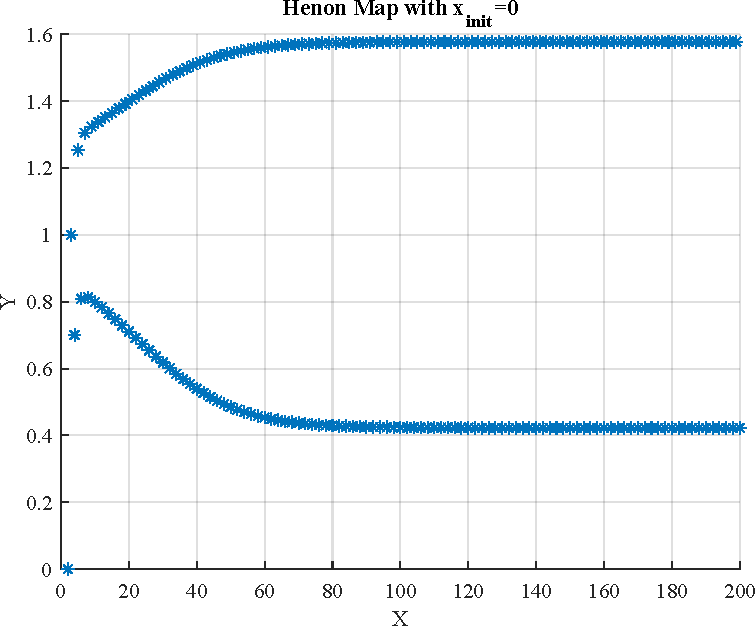
\includegraphics[width=\textwidth]{../Problem 3/prob3_x_init_0.pdf}
		\caption{}
	\end{subfigure}
	\hspace{1mm}
	\begin{subfigure}{.47\textwidth}
		\centering
		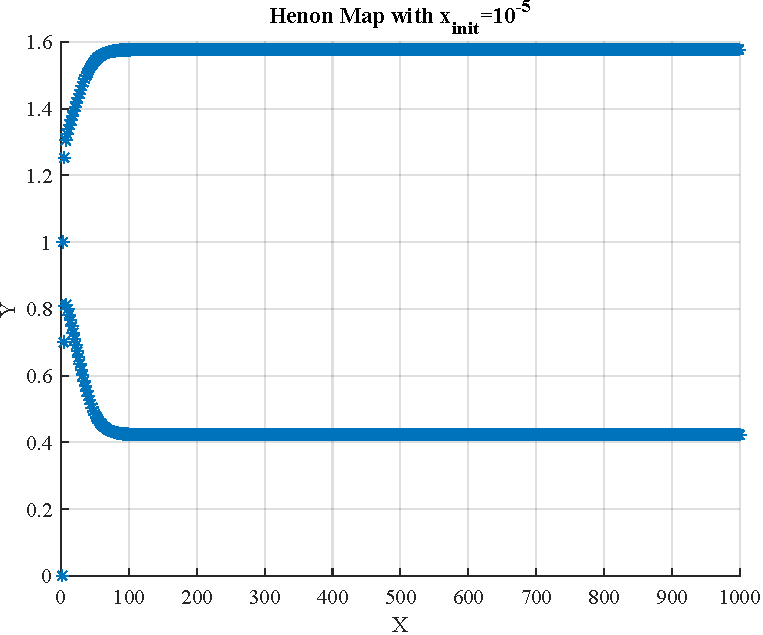
\includegraphics[width=\textwidth]{../Problem 3/prob3_x_init_1e-5.pdf}
		\caption{}
	\end{subfigure}
	\caption{Trajectories of Henon map's sequence with (a,b) = (0.3, 0.4)}
	\label{fig:prob3_x_init}
\end{figure}
From the produced plots, this system with parameters (0.3, 0.4) is periodic after converging.

\subsection{Multiple a values}
Figure~\ref{fig:prob3_multiple_a} shows output of the sequence for different values of $a$ and $b=0$. When $a \le 0.6$, the output swings for a bit and then stabilizes to a fixed number, with that number decreasing while $a$ approaches $0.6$.


\begin{figure}[htpb]
	\centering
	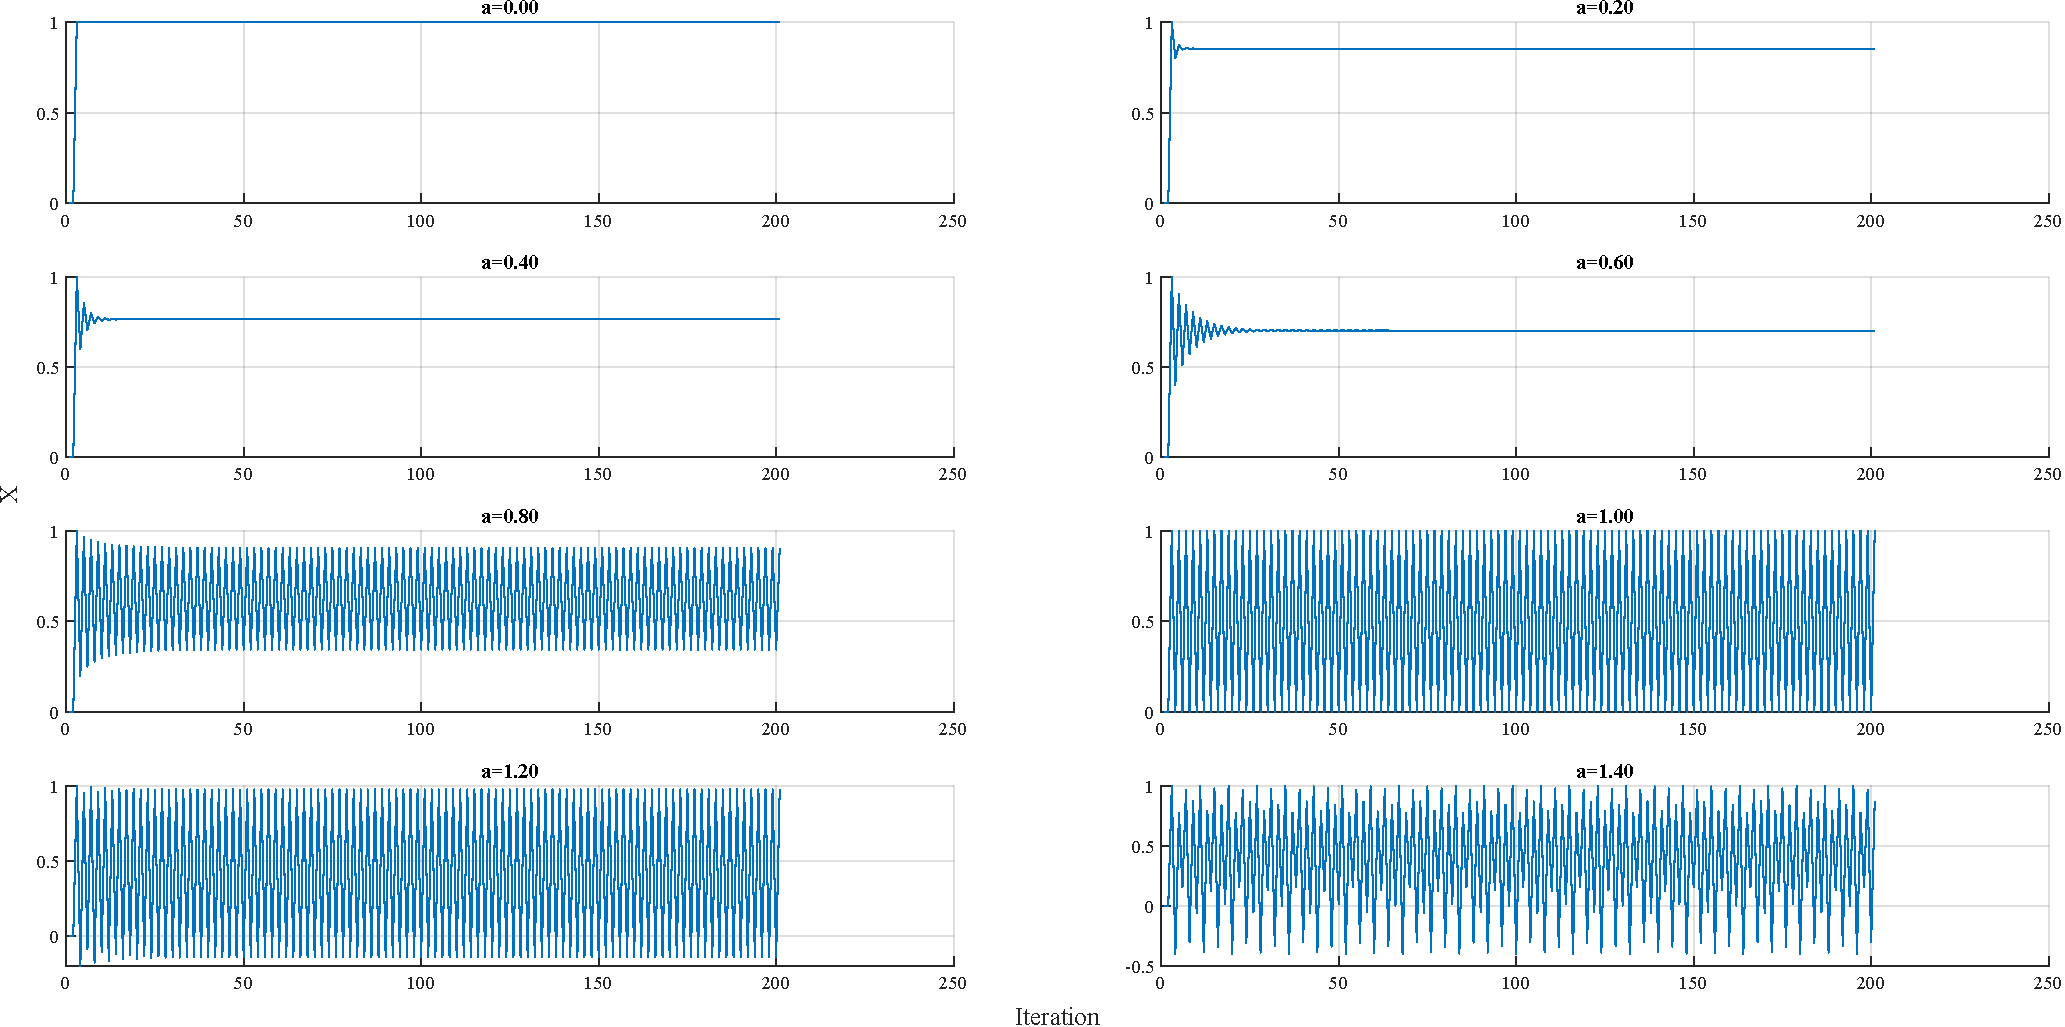
\includegraphics[width=\textwidth]{../Problem 3/prob3_(a)_multiple_a_b_0.pdf}
	\caption{Sequence output for different $a$ and $b=0$}
	\label{fig:prob3_multiple_a}
\end{figure}

When $a \ge 0.8$, output starts to oscillate. As $a$ approaches $1$, the oscillation's amplitude is getting bigger until it reaches value $1$.
After $a$ surpasses $1$, the oscillation starts to break down, as shown in the last two sub-figures. The greater $a$, the greater the disturbance on the oscillation thus chaos is created.

\subsection{Multiple initial x values}
